\documentclass{article}
\usepackage{tikz}
\pagestyle{empty}

\begin{document}
\colorbox{white}{%
    \tikzset{
        % �ı��ͱ߿�ľ���
        box/.style={inner sep=6pt}
    }
    \begin{tikzpicture}
        % �ڵ���״ �ڵ�ID �ڵ��ǩ
        %\draw[help lines] (10,10) grid (100, 100);
        \node[box] (tex) {.tex};
    \end{tikzpicture}

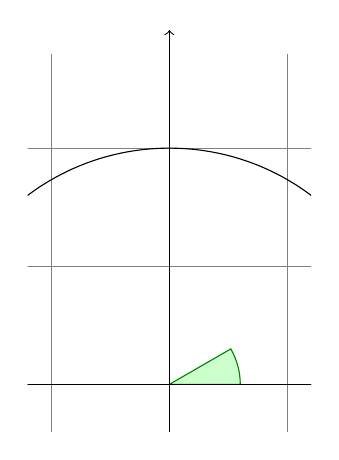
\begin{tikzpicture}[scale=3]
    \clip (-0.6,-0.2) rectangle (0.6,1.51);

    \draw[step=.5cm,help lines] (-1.4,-1.4) grid (1.4,1.4);

    \filldraw[fill=green!20,draw=green!50!black]
    (0,0) -- (3mm,0mm) arc (0:30:3mm) -- cycle;
    \draw[->] (-1.5,0) -- (1.5,0); \draw[->] (0,-1.5) -- (0,1.5);
    \draw (0,0) circle (1cm);
\end{tikzpicture}
}
\end{document} 
